% (find-LATEX "2020-1-C2-subst-trig-1.tex")
% (defun c () (interactive) (find-LATEXsh "lualatex -record 2020-1-C2-subst-trig-1.tex" :end))
% (defun C () (interactive) (find-LATEXsh "lualatex 2020-1-C2-subst-trig-1.tex" "Success!!!"))
% (defun D () (interactive) (find-pdf-page      "~/LATEX/2020-1-C2-subst-trig-1.pdf"))
% (defun d () (interactive) (find-pdftools-page "~/LATEX/2020-1-C2-subst-trig-1.pdf"))
% (defun e () (interactive) (find-LATEX "2020-1-C2-subst-trig-1.tex"))
% (defun u () (interactive) (find-latex-upload-links "2020-1-C2-subst-trig-1"))
% (defun v () (interactive) (find-2a '(e) '(d)))
% (defun cv () (interactive) (C) (ee-kill-this-buffer) (v) (g))
% (find-pdf-page   "~/LATEX/2020-1-C2-subst-trig-1.pdf")
% (find-sh0 "cp -v  ~/LATEX/2020-1-C2-subst-trig-1.pdf /tmp/")
% (find-sh0 "cp -v  ~/LATEX/2020-1-C2-subst-trig-1.pdf /tmp/pen/")
%   file:///home/edrx/LATEX/2020-1-C2-subst-trig-1.pdf
%               file:///tmp/2020-1-C2-subst-trig-1.pdf
%           file:///tmp/pen/2020-1-C2-subst-trig-1.pdf
% http://angg.twu.net/LATEX/2020-1-C2-subst-trig-1.pdf
% (find-LATEX "2019.mk")
% (find-C2-aula-links "2020-1-C2-subst-trig-1" "st1" "substtrig1")

% «.videos»			(to "videos")
%
% «.exemplo-1»			(to "exemplo-1")
% «.exercicio-1»		(to "exercicio-1")
% «.como-testar»		(to "como-testar")
% «.como-testar-exemplo»	(to "como-testar-exemplo")
% «.abreviacoes»		(to "abreviacoes")
% «.scans»			(to "scans")
% «.tan-e-sec-grande»		(to "tan-e-sec-grande")
% «.tan-e-sec-ids-e-blocos»	(to "tan-e-sec-ids-e-blocos")


% «videos»  (to ".videos")
% (find-ssr-links     "c2m201st1" "2020_C2_2020nov25_subst_trig_1")
% (code-eevvideo      "c2m201st1" "2020_C2_2020nov25_subst_trig_1")
% (code-eevlinksvideo "c2m201st1" "2020_C2_2020nov25_subst_trig_1")
% (find-c2m201st1video "0:00")

% (find-ssr-links     "c2m201tansec" "2020_subst_trig_tan_sec")
% (code-eevvideo      "c2m201tansec" "2020_subst_trig_tan_sec")
% (code-eevlinksvideo "c2m201tansec" "2020_subst_trig_tan_sec")
% (find-c2m201tansecvideo "0:00")




\documentclass[oneside,12pt]{article}
\usepackage[colorlinks,citecolor=DarkRed,urlcolor=DarkRed]{hyperref} % (find-es "tex" "hyperref")
\usepackage{amsmath}
\usepackage{amsfonts}
\usepackage{amssymb}
\usepackage{pict2e}
\usepackage[x11names,svgnames]{xcolor} % (find-es "tex" "xcolor")
%\usepackage{colorweb}                 % (find-es "tex" "colorweb")
%\usepackage{tikz}
%
% (find-dn6 "preamble6.lua" "preamble0")
%\usepackage{proof}   % For derivation trees ("%:" lines)
%\input diagxy        % For 2D diagrams ("%D" lines)
%\xyoption{curve}     % For the ".curve=" feature in 2D diagrams
%
\usepackage{edrx15}               % (find-LATEX "edrx15.sty")
\input edrxaccents.tex            % (find-LATEX "edrxaccents.tex")
\input edrxchars.tex              % (find-LATEX "edrxchars.tex")
\input edrxheadfoot.tex           % (find-LATEX "edrxheadfoot.tex")
\input edrxgac2.tex               % (find-LATEX "edrxgac2.tex")
%
%\usepackage[backend=biber,
%   style=alphabetic]{biblatex}            % (find-es "tex" "biber")
%\addbibresource{catsem-slides.bib}        % (find-LATEX "catsem-slides.bib")
%
% (find-es "tex" "geometry")
\usepackage[a6paper, landscape,
            top=1.5cm, bottom=.25cm, left=1cm, right=1cm, includefoot
           ]{geometry}
%
\begin{document}

\catcode`\^^J=10
\directlua{dofile "dednat6load.lua"}  % (find-LATEX "dednat6load.lua")

% %L dofile "edrxtikz.lua"  -- (find-LATEX "edrxtikz.lua")
% %L dofile "edrxpict.lua"  -- (find-LATEX "edrxpict.lua")
% \pu

% «defs»  (to ".defs")
% (find-LATEX "edrx15.sty" "colors-2019")
\long\def\ColorRed   #1{{\color{Red1}#1}}
\long\def\ColorViolet#1{{\color{MagentaVioletLight}#1}}
\long\def\ColorViolet#1{{\color{Violet!50!black}#1}}
\long\def\ColorGreen #1{{\color{SpringDarkHard}#1}}
\long\def\ColorGreen #1{{\color{SpringGreenDark}#1}}
\long\def\ColorGreen #1{{\color{SpringGreen4}#1}}
\long\def\ColorGray  #1{{\color{GrayLight}#1}}
\long\def\ColorGray  #1{{\color{black!30!white}#1}}
\long\def\ColorBrown #1{{\color{Brown}#1}}
\long\def\ColorBrown #1{{\color{brown}#1}}

\long\def\ColorShort #1{{\color{SpringGreen4}#1}}
\long\def\ColorLong  #1{{\color{Red1}#1}}

\def\frown{\ensuremath{{=}{(}}}
\def\True {\mathbf{V}}
\def\False{\mathbf{F}}
\def\D    {\displaystyle}

\def\drafturl{http://angg.twu.net/LATEX/2020-1-C2.pdf}
\def\drafturl{http://angg.twu.net/2020.1-C2.html}
\def\draftfooter{\tiny \href{\drafturl}{\jobname{}} \ColorBrown{\shorttoday{} \hours}}

% (find-angg ".emacs" "c2q192")


%  _____ _ _   _                               
% |_   _(_) |_| | ___   _ __   __ _  __ _  ___ 
%   | | | | __| |/ _ \ | '_ \ / _` |/ _` |/ _ \
%   | | | | |_| |  __/ | |_) | (_| | (_| |  __/
%   |_| |_|\__|_|\___| | .__/ \__,_|\__, |\___|
%                      |_|          |___/      
%
% «title»  (to ".title")

\thispagestyle{empty}

\begin{center}

\vspace*{1.2cm}

{\bf \Large Cálculo 2 - 2020.1}

\bsk

Aula 19: Substituição trigonométrica

\bsk

Eduardo Ochs - RCN/PURO/UFF

\url{http://angg.twu.net/2020.1-C2.html}

\end{center}

\newpage

%\printbibliography

% «exemplo-1»  (to ".exemplo-1")
% (c2m201substtrig1p 2 "exemplo-1")
% (c2m201substtrig1    "exemplo-1")

{\bf Primeiro exemplo (só o início)}

% (find-latexscan-links           "C2" "20201125_160341_substituicao_s")
% (find-xpdf-page    "~/LATEX/2020-1-C2/20201125_160341_substituicao_s.pdf")
%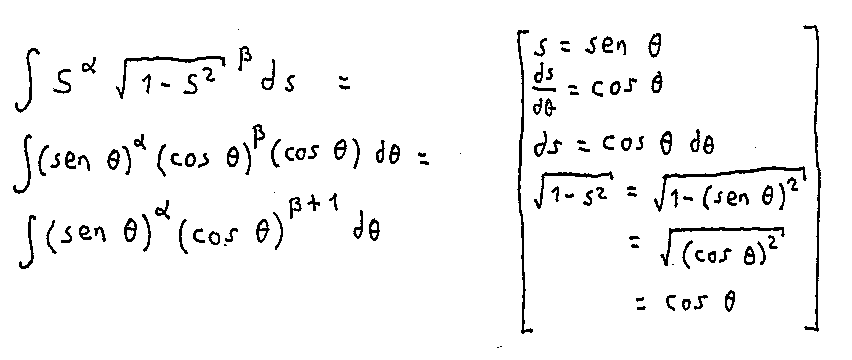
\includegraphics[height=8cm]{2020-1-C2/20201125_160341_substituicao_s.pdf}
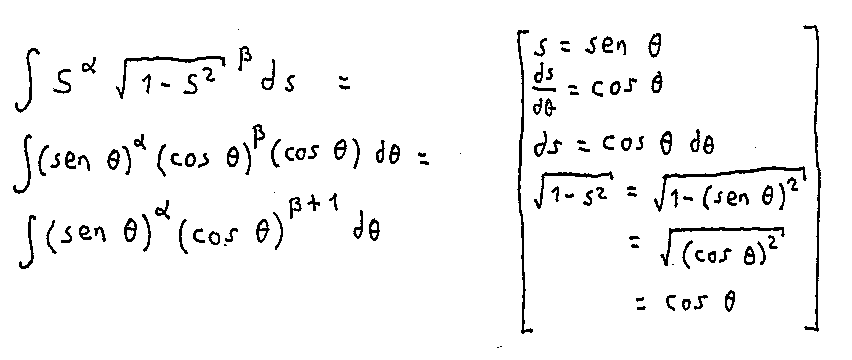
\includegraphics[width=11cm]{2020-1-C2/20201125_160341_substituicao_s.pdf}

Pra resolver isto você vai precisar da técnica que a gente viu

na ``Aula 18: Integrais de potências de senos e cossenos''.

% (c2m201ipscp 4 "exemplo-2")
% (c2m201ipsc    "exemplo-2")


\newpage

% «exercicio-1»  (to ".exercicio-1")
% (c2m201substtrig1p 3 "exercicio-1")
% (c2m201substtrig1    "exercicio-1")

{\bf Exercício 1}

% (find-latexscan-links "C2" "20201125_160159_exerc_1")
% (find-xpdf-page   "~/LATEX/2020-1-C2/20201125_160159_exerc_1.pdf")
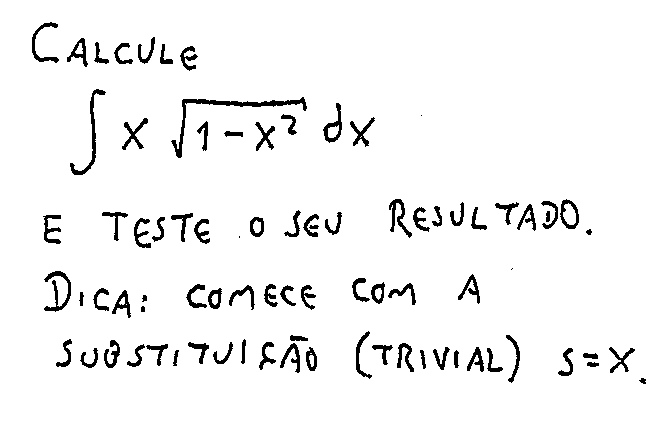
\includegraphics[width=11cm]{2020-1-C2/20201125_160159_exerc_1.pdf}

% (find-es "ipython" "2020.1-int-subst")


\newpage

% «como-testar»  (to ".como-testar")
% (c2m201tfc22p 2 "integral-indefinida")
% (c2m201tfc22    "integral-indefinida")

{\bf Como testar a sua integral?}

\ssk

Lembre que pra testar se uma igualdade como $\intx{f(x)} = F(x)$

é verdade a gente ``deriva os dois lados''... eu costumo escrever

um teste destes assim,
%
\def\qeq{\overset{?}{=}}
%
$$\begin{array}{ccr}
  \displaystyle \int {f(x)} \, dx &\qeq& F(x) \\
                f(x)  &\qeq& \frac{d}{dx} F(x) \\
  \end{array}
$$

e aí eu calculo a derivada $\frac{d}{dx} F(x)$ usando `$=$'s sem `?'.

Se eu chegar a um resultado igual a $f(x)$ então concluo que os

`$\qeq$'s são verdade e se eu chegar a algo que é evidentemente

diferente de $f(x)$ eu concluo que os `$\qeq$'s são falsos.

\ssk

Tem dois exemplos no próximo slide.

\newpage

% «como-testar-exemplo»  (to ".como-testar-exemplo")
% (c2m201substtrig1p 5 "como-testar-exemplo")
% (c2m201substtrig1    "como-testar-exemplo")

% (find-latexscan-links "C2" "20201126_strig_teste")
% (find-xpdf-page "~/LATEX/2020-1-C2/20201126_strig_teste.pdf")
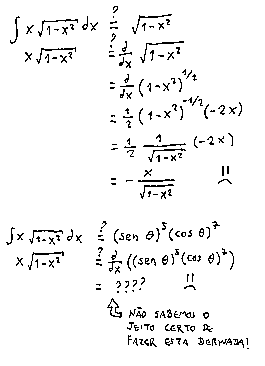
\includegraphics[height=8cm]{2020-1-C2/20201126_strig_teste.pdf}

\newpage

% «abreviacoes»  (to ".abreviacoes")
% (c2m201substtrig1p 6 "abreviacoes")
% (c2m201substtrig1    "abreviacoes")

{\bf Abreviações}

\ssk

A partir de agora nós \ColorRed{às vezes} vamos usar certas
abreviações, como por exemplo ``$s = \sen θ$''... só que essas
abreviações dão \ColorRed{muita} margem pra erro a não ser que a gente
saiba testar muito bem o que a gente está fazendo...

O truque pra fazer esses testes é o seguinte. Vamos ter que definir
duas linguagens diferentes --- a ``linguagem sem abreviações'' e a
``linguagem com abreviações'' e pra testar se algo na ``linguagem
\ColorRed{com} abreviações'' faz sentido nós vamos ter que traduzí-lo
pra ``linguagem \ColorRed{sem} abreviações'' e ver se ele faz sentido
lá.

\newpage

{\bf Abreviações (2)}

\ssk

As contas do ``primeiro exemplo'' no slide 2 estão todas feitas na
linguagem sem abreviações. Quando o $s$ aparece ele é sempre uma outra
variável, nova, e diferente da variável anterior, que é $θ$. Cada
expressão que aparece ou é toda na variável $s$ ou toda na variável
$θ$, inclusive no bloquinho de substituições... exceto pela segunda
linha dele, que é ``$\frac{ds}{dθ} = \cos θ$'', e que eu estou
avisando desde o início que é uma gambiarra --- esta linha deve ser
interpretada como $\frac{d}{dθ} \senθ = \cosθ$''.

\newpage

{\bf Abreviações (3)}

\ssk

Outra coisa importante: no vídeo eu enfatizo bastante que nos
bloquinhos de substituições que estamos usando para integração por
substituição de variáveis a primeira linha é algo como ``$v = expr$'',
onde $v$ é uma \ColorRed{variável nova} e $expr$ é uma {\sl expressão
  na variável antiga}, e \ColorRed{todas as outras linhas vão ser
  consequências da primeira}. A gente vai fazer isso sempre --- e aí
pra conseguir resolver o exercício 1 você vai precisar de três
bloquinhos de substituição \ColorRed{separados}...

\begin{itemize}

\item o primeiro começa com ``$s=x$'',

\item o segundo começa com ``$\sen θ = s$''. Alguns livros que fazem
  os detalhes com todo o cuidado mostram que esse passo na verdade é
  uma substituição ``$θ=\arcsen s$'' disfarçada, e que isso é uma
  ``substituição inversa''...

\item o terceiro bloquinho de substituição começa ou com ``$c = \cos
  θ$'' ou com ``$s = \sen θ$''... veja os slides da ``Aula 18:
  Integrais de potências de senos e cossenos'', em especial a dica no
  último slide.

% (c2m201ipscp)
% (c2m201ipsc)
% (c2m201ipscp 6 "pares-e-impares")
% (c2m201ipsc    "pares-e-impares")

\end{itemize}





% Nesse momento do curso ainda e' proibido usar s como abreviacao pra
% sen x. A gente so' vai poder usar essas abreviacoes quando a gente
% souber expandir elas exatamente do jeito certo pra obter expressoes
% que fazem sentido na linguagem sem as abreviacoes. Vou fazer um slide
% explicando isso... se a gente usar essas abreviacoes sem saber
% MUUUUITO bem o que a gente esta' fazendo a gente acaba errando as
% contas quase todas. Acho que fica mais claro - e voce vai ter menos
% risco de errar - se voce fizer as duas substituicoes em bloquinhos
% separados... a primeira e' x=theta e a segunda e' s = sen theta
% 
% Matheus Casagrande
% x=theta?
% Eduardo Ochsadmin
% sim
% uma "mudanca de variavel trivial"
% mais facil ainda do que x = 2 theta + 3
% e se voce for usar c = cos theta voce ainda vai precisar de outro bloquinho
% 
% Matheus Casagrande
% mas nao seria x = sen(theta)?
% Eduardo Ochsadmin
% depende do que voce esta' querendo fazer
% tenta, x= sen(theta) vai dar certo tambem
% mas a dica e' que cada bloquinho de substituicoes para a integracao por substituicao comeca com
% 
% Matheus Casagrande
% mas era o que eu estava tentando e aparentemente estava errado
% Eduardo Ochsadmin
% variavelnova = expressaonavariavelantiga
% e todo o resto e' consequencia disso
% entao eu te ajudo com isso assim que eu voltar! ate' ja'!
% 
% Matheus Casagrande
% ok ate mais


% {\bf Abreviações}

% (find-latexscan-links "C2" "20201125_160249_abreviacoes")
% (find-xpdf-page "~/LATEX/2020-1-C2/20201125_160249_abreviacoes.pdf")
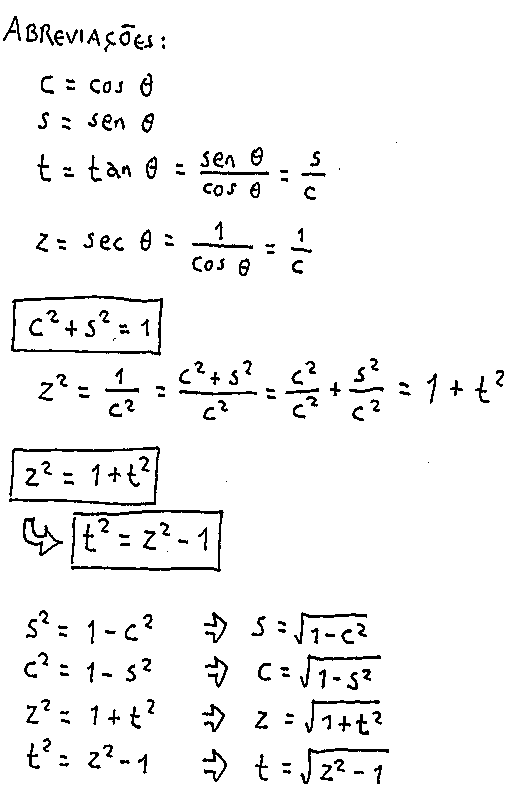
\includegraphics[height=8cm]{2020-1-C2/20201125_160249_abreviacoes.pdf}
%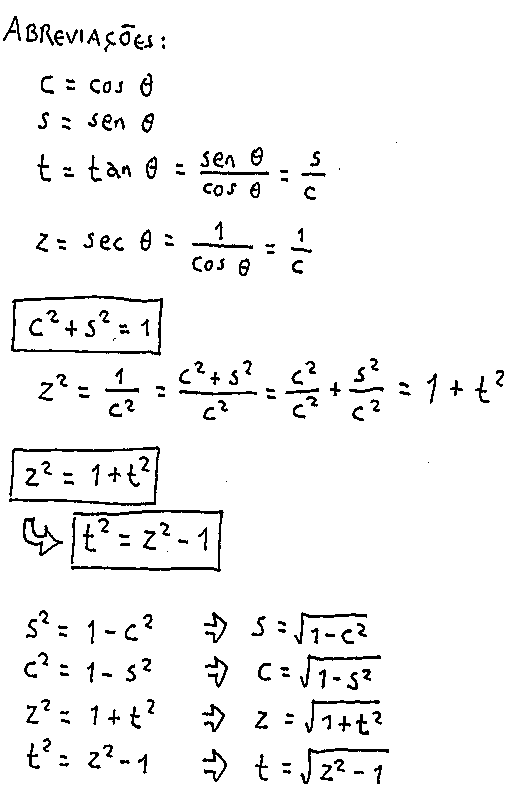
\includegraphics[width=11cm]{2020-1-C2/20201125_160249_abreviacoes.pdf}

\newpage

As explicações (de tudo até aqui) estão neste vídeo:

\ssk

\url{http://angg.twu.net/eev-videos/2020_C2_2020nov25_subst_trig_1.mp4}

\bsk
\bsk

As páginas seguintes têm o que a gente precisa saber pra trabalhar com
os outros dois tipos de substituições trigonométricas. \ColorRed{Estou
  fazendo um vídeo sobre elas! Link em breve!}


\newpage

% «tan-e-sec-grande»  (to ".tan-e-sec-grande")
% (c2m201substtrig1p 12 "tan-e-sec-grande")
% (c2m201substtrig1    "tan-e-sec-grande")

% (find-latexscan-links "C2" "20201202_substtrig_grande")
% (find-xpdf-page "~/LATEX/2020-1-C2/20201202_substtrig_grande.pdf")
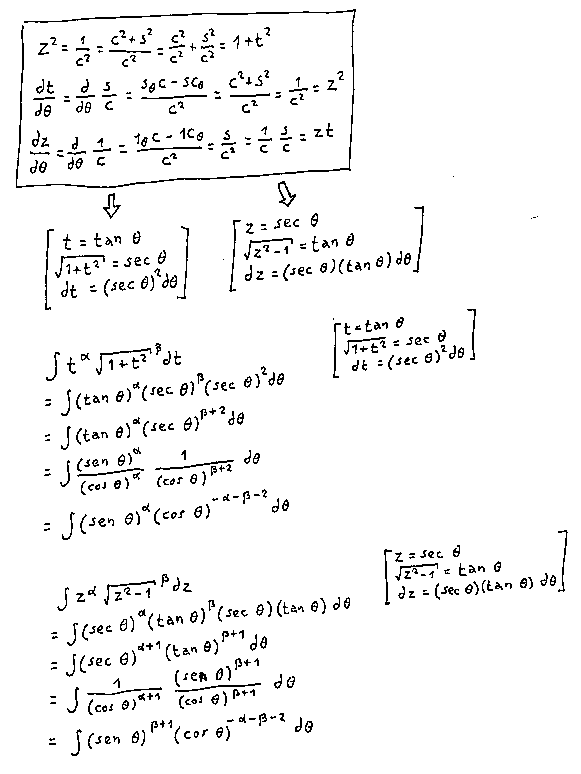
\includegraphics[height=8cm]{2020-1-C2/20201202_substtrig_grande.pdf}
%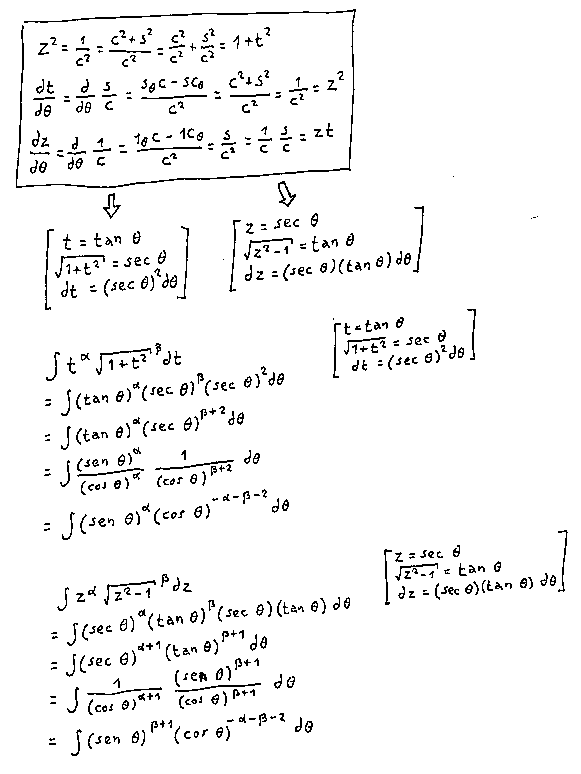
\includegraphics[width=11cm]{2020-1-C2/20201202_substtrig_grande.pdf}

\newpage

% «tan-e-sec-ids-e-blocos»  (to ".tan-e-sec-ids-e-blocos")
% (find-latexscan-links "C2" "20201202_substtrig_ids_e_blocos")
% (find-xpdf-page "~/LATEX/2020-1-C2/20201202_substtrig_ids_e_blocos.pdf")
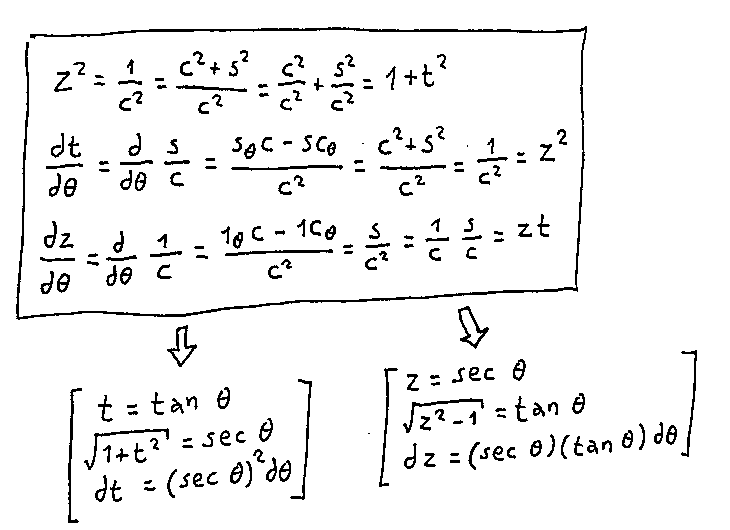
\includegraphics[height=8cm]{2020-1-C2/20201202_substtrig_ids_e_blocos.pdf}
%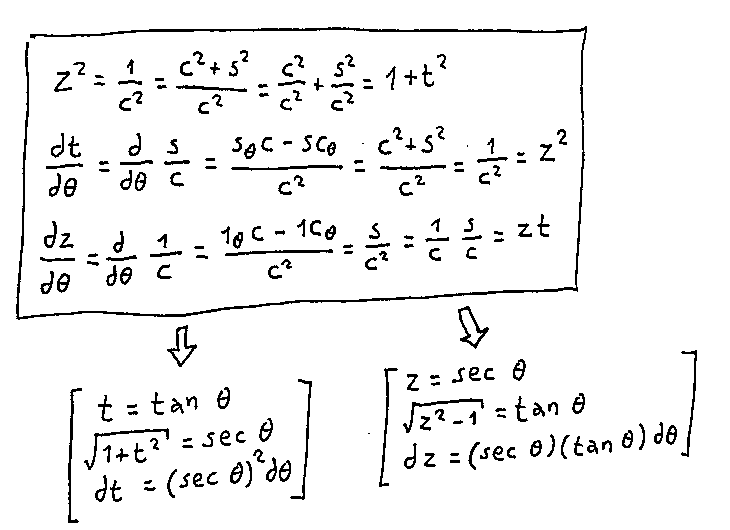
\includegraphics[width=11cm]{2020-1-C2/20201202_substtrig_ids_e_blocos.pdf}

\newpage

% (find-latexscan-links "C2" "20201202_substtrig_t")
% (find-xpdf-page "~/LATEX/2020-1-C2/20201202_substtrig_t.pdf")
%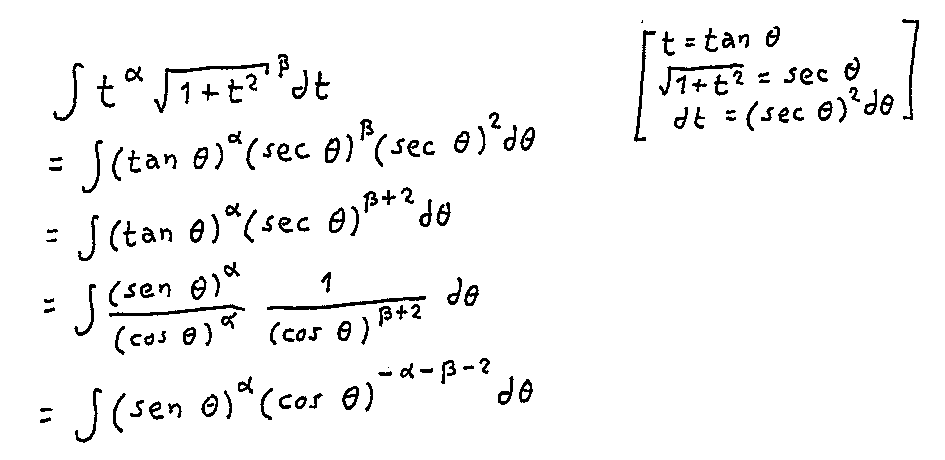
\includegraphics[height=8cm]{2020-1-C2/20201202_substtrig_t.pdf}
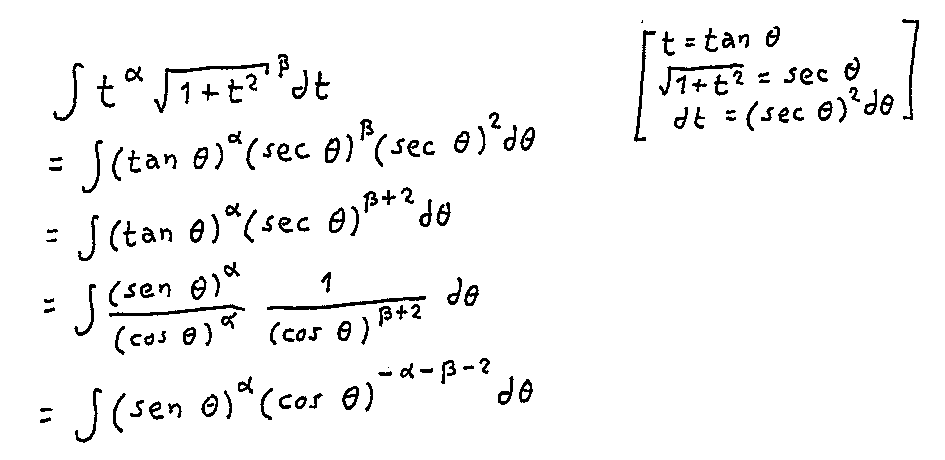
\includegraphics[width=11cm]{2020-1-C2/20201202_substtrig_t.pdf}

\newpage

% (find-latexscan-links "C2" "20201202_substtrig_z")
% (find-xpdf-page "~/LATEX/2020-1-C2/20201202_substtrig_z.pdf")
%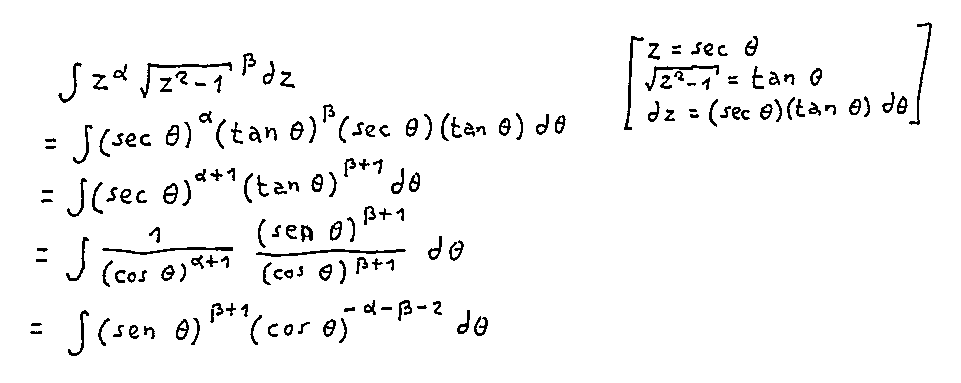
\includegraphics[height=8cm]{2020-1-C2/20201202_substtrig_z.pdf}
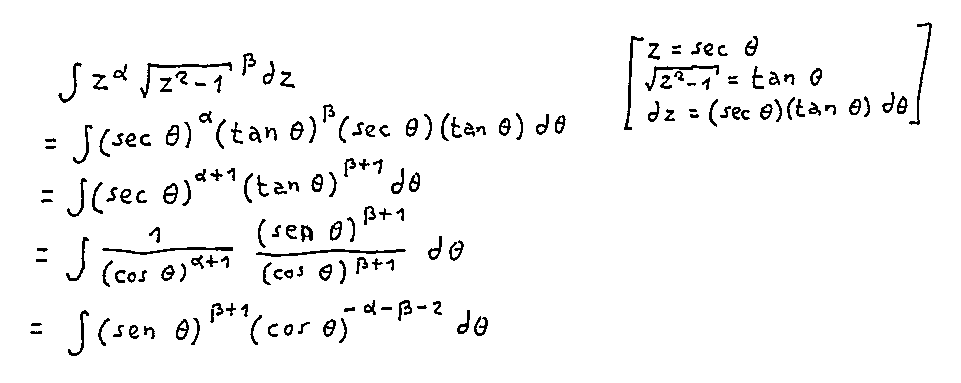
\includegraphics[width=11cm]{2020-1-C2/20201202_substtrig_z.pdf}



%L print(); print("Success!!!")
\pu

\end{document}

 (eepitch-shell)
 (eepitch-kill)
 (eepitch-shell)
cp -v  ~/LATEX/2020-1-C2-subst-trig-1.pdf /tmp/
cd /tmp/
xournalpp      2020-1-C2-subst-trig-1.pdf



%  ____                      
% / ___|  ___ __ _ _ __  ___ 
% \___ \ / __/ _` | '_ \/ __|
%  ___) | (_| (_| | | | \__ \
% |____/ \___\__,_|_| |_|___/
%                            
% «scans»  (to ".scans")
% (find-LATEX "2020-1-C3-aprox-2a-ordem-R2.tex" "scans")

 (eepitch-shell)
 (eepitch-kill)
 (eepitch-shell)
# (find-fline "~/2020.1-C2/")
# (find-fline "/tmp/c2trigsubst1/")
# (find-fline "/tmp/substtrig/")
# (find-fline "~/LATEX/2020-1-C3/")
cd /tmp/qc3/
cd /tmp/c2trigsubst1/
cd /tmp/
cd /tmp/substtrig/
f () { rm -fv $1.png $1.pdf; djvuize $1.pdf }
f () { rm -fv $1.png $1.pdf; djvuize WHITEBOARDOPTS="-m 0.5" $1.pdf; xpdf $1.pdf }
f () { rm -fv $1.png $1.pdf; djvuize WHITEBOARDOPTS="-m 0.25" $1.pdf; xpdf $1.pdf }
f () { cp -fv $1.png $1.pdf       ~/2020.1-C3/ }
f () { cp -fv        $1.pdf ~/LATEX/2020-1-C3/ }
f () { cp -fv $1.png $1.pdf       ~/2020.1-C2/
       cp -fv        $1.pdf ~/LATEX/2020-1-C2/
       cat <<%%%
% (find-latexscan-links "C2" "$1")
%%%
}

f 20201202_substtrig_grande
f 20201202_substtrig_ids_e_blocos
f 20201202_substtrig_t
f 20201202_substtrig_z

f 20201126_strig_teste

f 20201125_160159_exerc_1
f 20201125_160249_abreviacoes
f 20201125_160341_substituicao_s


 (eepitch-shell)
 (eepitch-kill)
 (eepitch-shell)
cp -v  ~/LATEX/2020-1-C2-subst-trig-1.pdf /tmp/
cd /tmp/
xournalpp 2020-1-C2-subst-trig-1.pdf


%  __  __       _        
% |  \/  | __ _| | _____ 
% | |\/| |/ _` | |/ / _ \
% | |  | | (_| |   <  __/
% |_|  |_|\__,_|_|\_\___|
%                        
% <make>

 (eepitch-shell)
 (eepitch-kill)
 (eepitch-shell)
# (find-LATEXfile "2019planar-has-1.mk")
make -f 2019.mk STEM=2020-1-C2-subst-trig-1 veryclean
make -f 2019.mk STEM=2020-1-C2-subst-trig-1 pdf

% Local Variables:
% coding: utf-8-unix
% ee-tla: "c2m201substtrig1"
% End:
